\subsection{Теорема о художественной галерее}

\textbf{Задача.} Сколько сторожей надо расставить в углах произвольного $n$-угольника, чтобы каждую внутреннюю точку видел кто-то из них?

\begin{lemma}
    \label{lem:treang}
    Всякий многоугольник можно диагоналями разбить на треугольники, причем полученный граф раскрашивается в $3$ цвета.
\end{lemma}

\begin{proof}
    
    Индукция по числу сторон $n$.

    \textsl{База:} $n = 3$, треугольник --- уже разбит. Раскашивается.

    \textsl{Переход:} находим угол меньше $180^\circ$, он есть.

    \begin{itemize}
        \item Если отрезок между соседними с ним вершинами лежит внутри многоугольника:
        \begin{itemize}
            \item Отрезаем треугольник
            \item По индукции, все остальное разбивается и раскрашивается.
            \item Отрезанная вершина раскрашивается в свободный цвет.
        \end{itemize}

        \item Если этот отрезок пересекает какие-то другие отрезки:
        \begin{itemize}
            \item Проводим отрезок из вершины угла к концу одного из мешающих отрезков (можно выбрать, например, конец отрезка внутри угла ближайший к вершине), разбиваем многоугольник на два.
            \item Каждая половина разбивается и раскрашивается.
            \item Цвета в одной из половин переименовываются, чтобы на общем отрезке были те же два цвета.
        \end{itemize}
    \end{itemize}
\end{proof}

\begin{theorem}[Хватал, 1975]~
    
    Для всякого $n \geq 3$ в любом $n$-угольнике достаточно $\lfloor \frac{n}{3} \rfloor$ сторожей, расставленных в вершинах.

    Существует $n$-угольник, для которого необходимо не менее $\lfloor \frac{n}{3} \rfloor$ сторожей, даже если разрешить их расстановку в произвольных точках.

\end{theorem}

Нижняя оценка --- гребенка Хватала: $n = 3k$, минимум $k$ сторожей.

\begin{center}
    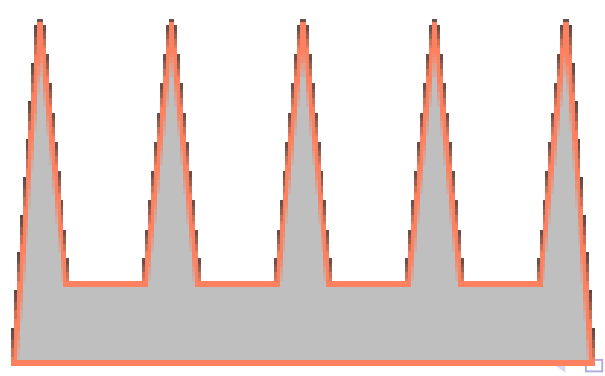
\includegraphics[width=0.5\textwidth]{par26hvat.png}
\end{center}

\begin{proof}
    
    По лемме \ref*{lem:treang} строим разбиение на треугольники так, что полученный граф раскрашивается в три цвета.

    Из этих цветов выбираем тот, который используется не чаще других; им раскрашено вершин $\lfloor \frac{n}{3} \rfloor$.
    
    Расставляем сторожей в вершинах, раскрашенных этим цветом. 

    У каждого треугольника есть сторож в одной из его вершин, значит видно любую точку внутри любого треугольника, а значит и многоугольника.
\end{proof}